% Lecture Template for ME3001-001-Tristan Hill - Spring 2017 - Fall 2018
% 
% Mechanical Engineering Analysis with MATLAB
%
% Systems of Linear Equations - Lecture 1


% Document settings
\documentclass[11pt]{article}
\usepackage[margin=1in]{geometry}
\usepackage[pdftex]{graphicx}
\usepackage{multirow}
\usepackage{setspace}
\usepackage{hyperref}
\usepackage{color,soul}
\usepackage{fancyvrb}
\usepackage{framed}
\usepackage{wasysym}
\usepackage{multicol}

\pagestyle{plain}
\setlength\parindent{0pt}
\hypersetup{
    bookmarks=true,         % show bookmarks bar?
    unicode=false,          % non-Latin characters in Acrobat’s bookmarks
    pdftoolbar=true,        % show Acrobat’s toolbar?
    pdfmenubar=true,        % show Acrobat’s menu?
    pdffitwindow=false,     % window fit to page when opened
    pdfstartview={FitH},    % fits the width of the page to the window
    pdftitle={My title},    % title
    pdfauthor={Author},     % author
    pdfsubject={Subject},   % subject of the document
    pdfcreator={Creator},   % creator of the document
    pdfproducer={Producer}, % producer of the document
    pdfkeywords={keyword1} {key2} {key3}, % list of keywords
    pdfnewwindow=true,      % links in new window
    colorlinks=true,       % false: boxed links; true: colored links
    linkcolor=red,          % color of internal links (change box color with linkbordercolor)
    citecolor=green,        % color of links to bibliography
    filecolor=magenta,      % color of file links
    urlcolor=blue           % color of external links
}

% assignment number 

\definecolor{mygreen}{rgb}{0, .39, 0}

%\definecolor{dred}{#8B0000}
% [153,50,204] - dark orchid
\definecolor{mypurple}{rgb}{0.6,0.1961,0.8}
%[139,69,19] - saddle brown
\definecolor{mybrown}{rgb}{0.5451,0.2706,0.0745}

\definecolor{mygray}{rgb}{.6, .6, .6}

\setulcolor{red} 
\setstcolor{green} 
\sethlcolor{mygray} 

\newcommand{\VA}{\vspace{2mm}}
\newcommand{\VB}{\vspace{5mm}} 
\newcommand{\VC}{\vspace{30mm}} 
 
\newcommand{\R}{\color{red}}
\newcommand{\B}{\color{blue}}
\newcommand{\K}{\color{black}}
\newcommand{\G}{\color{mygreen}}
\newcommand{\PR}{\color{mypurple}}

\newcommand{\NUM}{1} 
\newcommand{\VSpaceSize}{2mm} 
\newcommand{\HSpaceSize}{2mm} 

\begin{document}

\textbf{ \LARGE FE Review - Solid Mechanics - Statics} \\\\
\textbf{ \LARGE Review of vector mechanics and loads analysis } \\

\begin{itemize}

	\item  \textbf{\LARGE Example 1}:\\
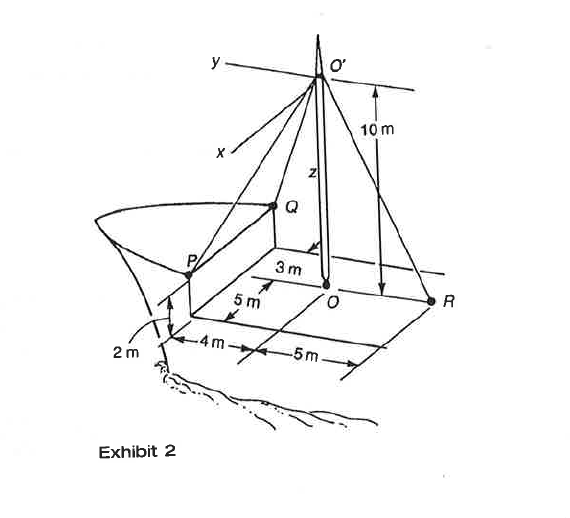
\includegraphics[scale=.75]{lecture1_fig1.png}
		\LARGE
		\begin{enumerate}
			\item Determine the lengths of the guylines O'P and O'Q and the angle between them.\\

			\item Suppose the guy line P'P has a tension of 800N. What is the moment from this force about O?

		\end{enumerate}

\newpage
	\item  \textbf{\LARGE Example 2}:\\
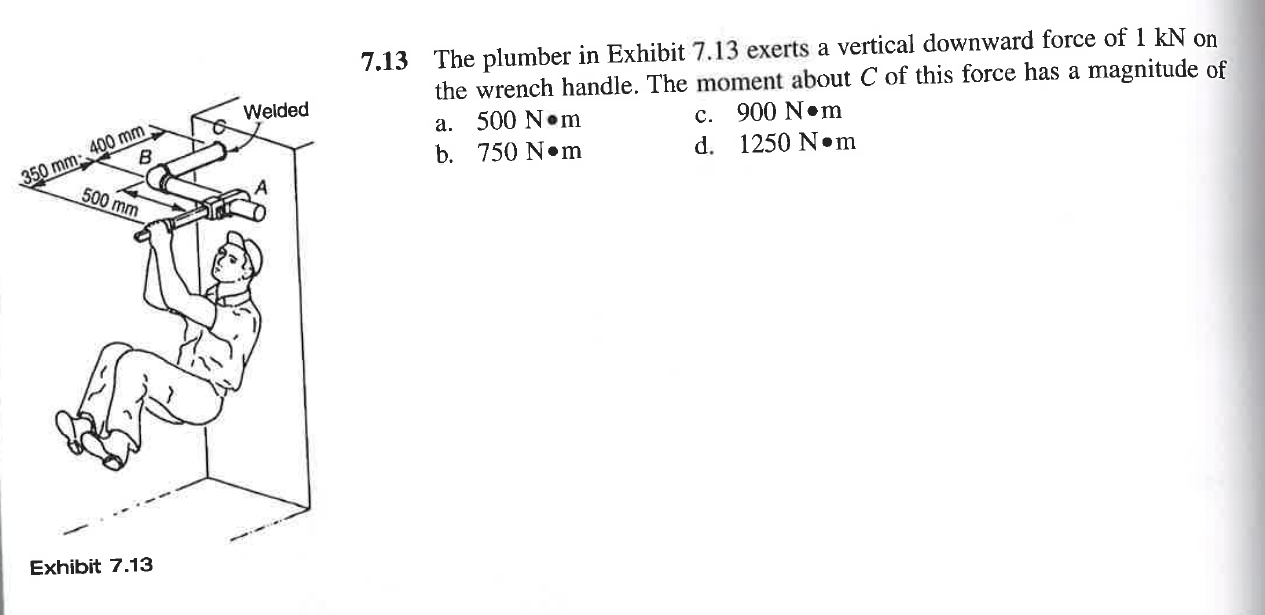
\includegraphics[scale=.5]{lecture1_fig2.png}
		\LARGE

\newpage		
	\item  \textbf{\LARGE Example 3}:\\
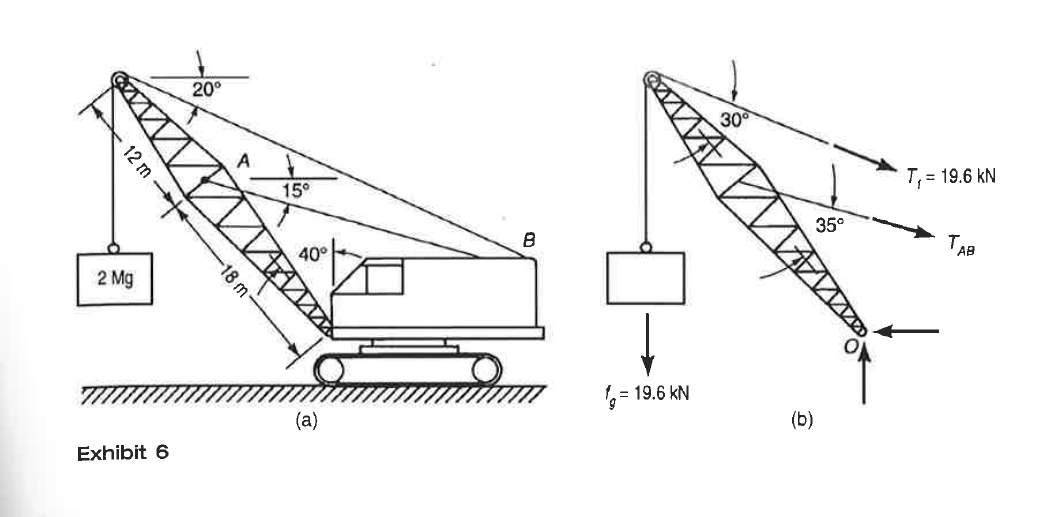
\includegraphics[scale=.5]{lecture1_fig3.png}
		\LARGE
				\begin{enumerate}
			\item Neglecting all loads except the 2Mg load, find the tension in cable AB.\\



		\end{enumerate}

		
\end{itemize}
\newpage

	

\end{document}



